\subsection{Filtration and topology of the ring W(A)}

Lemma 4. --- Let A be a ring and let \(m \geqslant 1\) be an integer. One has

\[
\boldsymbol {a} = \left(a _ {0}, \dots , a _ {m - 1}, 0, \dots\right) + \underbrace {\left(0 , \dots , 0 , \right.} _ {m \text { terms }}, a _ {m}, a _ {m + 1}, \dots)\tag{34}
\]

for all a in W(A).

Let \(\rho: B \to A\) be a ring homomorphism satisfying the conditions of lemma 3 of no. 4. Then \(W(\rho): W(B) \to W(A)\) is a surjective ring homomorphism, and \(\Phi_B: W(B) \to B^N\) is an injective homomorphism. It therefore suffices to prove that one has

\[
\Phi_ {n} (\boldsymbol {b}) = \Phi_ {n} (b _ {0},..., b _ {m - 1}, 0,...) + \Phi_ {n} (0,..., 0, b _ {m}, b _ {m + 1},...) \tag{35}
\]

for all b in W(B) and all integers \(m \geqslant 1, n \geqslant 0\) . Now one has

\[
\begin{array}{r l} \Phi_ {n} (b _ {0},..., b _ {m - 1},... \dots) & = \Phi_ {n} (b _ {0},..., b _ {n}) \quad \text { if } \quad 0 \leqslant n <   m \\ & = \sum_ {i = 0} ^ {m - 1} p ^ {i}. b _ {i} ^ {p ^ {n - i}} \quad \text { if } \quad m \leqslant n \end{array}
\]

\[
\begin{array}{r l} \Phi_ {n} (0, \dots , 0, b _ {m}, b _ {m + 1}, \dots) & = 0 \\ & = \sum_ {i = m} ^ {n} p ^ {i}. b _ {i} ^ {p ^ {n - i}} \end{array} \quad \text { if } \quad 0 \leqslant n <   m \quad \text { if } \quad m \leqslant n,
\]

whence formula (35).

Let A be a ring. For every integer \(m \geqslant 0\) , denote by \(\mathbf{V}_{m}(\mathbf{A})\) the set of Witt vectors \(\boldsymbol{a} = (a_{n})_{n \in \mathbb{N}}\) such that \(a_{n} = 0\) for \(0 \leqslant n < m\) . It is the image of the \(m\)-th power \(\mathbf{V}^{m}\) of the map \(\mathbf{V}_{\mathrm{A}}\) . The formulas

\begin{enumerate}
\def\labelenumi{(\arabic{enumi})}
\setcounter{enumi}{35}
\tightlist
\item
\end{enumerate}

\[
\mathrm{V} ^ {m} (\boldsymbol {a} + \boldsymbol {b}) = \mathrm{V} ^ {m} (\boldsymbol {a}) + \mathrm{V} ^ {m} (\boldsymbol {b})\tag{37}
\]

\[
\mathrm{V} ^ {m} (a) \times b = \mathrm{V} ^ {m} (a \times \mathrm{F} ^ {m} (b))
\]

result from prop. 3 of no. 5 by induction on m. They imply that V \(_{m}\) (A) is an ideal of W(A).

\pandocbounded{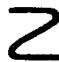
\includegraphics[keepaspectratio]{images/part001_18cee607.jpg}}

One sets \(\mathrm{V}_{m}(\mathrm{A}) = \mathrm{W}(\mathrm{A})\) if \(m < 0\) . The sequence \((\mathrm{V}_{m}(\mathrm{A}))_{m \in \mathbf{Z}}\) is a decreasing filtration on the additive group of the ring \(\mathrm{W}(\mathrm{A})\) . It is compatible with the ring structure of \(\mathrm{W}(\mathrm{A})\) (III, § 2, no. 1, def. 2) if and only if A is a ring of characteristic \(p\) (cf. no. 3, example 2 and infra, no. 8, corollary of prop. 5).

In what follows, one endows W(A) with the topology \(\mathcal{G}\) associated with the filtration \((\mathrm{V}_m(\mathrm{A}))_{m\in \mathbf{Z}}\) . Since \(\mathrm{V}_m(\mathrm{A})\) is an ideal of W(A) for all \(m\in \mathbf{Z}\) , the topology \(\mathcal{G}\) is compatible with the ring structure of W(A) (TG, III, p. 49, example 3). Let \(a\in \mathrm{W(A)}\) ; the sets \(a + \mathrm{V}_m(\mathrm{A})\) , where \(m\) runs through N, form a fundamental system of neighborhoods of \(a\) for \(\mathcal{G}\) . Now, it follows from lemma 4 that \(a + \mathrm{V}_m(\mathrm{A})\) consists of the Witt vectors \(b\) such that \(a_i = b_i\) for \(0\leqslant i < m\) . Consequently, \(\mathcal{G}\) is none other than the product topology on \(\mathbf{A}^{\mathbf{N}}\) of the discrete topology on each of the factors, and W(A) is therefore a separated and complete topological ring (TG, II, p. 17, prop. 10 and TG, III, p. 22, prop. 4).

Denote by \(\tau_{\mathbf{A}}\) (or simply \(\tau\) ) the map from A to W(A) which associates \((a, 0, 0, \ldots)\) with each element \(a\) of A. We have \(\Phi_n(\tau(a)) = a^{p^n}\) for every \(n \in \mathbb{N}\) . For every ring homomorphism \(\rho: \mathbf{B} \to \mathbf{A}\) , one has W( \(\rho\) ) \(\circ\) \(\tau_{\mathbf{B}} = \tau_{\mathbf{A}} \circ \rho\) .

PROPOSITION 4. --- Let \(a\) and \(b\) be in \(\mathbf{A}\) and let \(\boldsymbol{x} = (x_n)_{n \in \mathbb{N}}\) be an element of \(\mathbf{W}(\mathbf{A})\) .

\begin{enumerate}
\def\labelenumi{\alph{enumi})}
\tightlist
\item
  One has the formulas
\end{enumerate}

\begin{enumerate}
\def\labelenumi{(\arabic{enumi})}
\setcounter{enumi}{37}
\tightlist
\item
\end{enumerate}

\[
\tau (a b) = \tau (a) \times \tau (b)\tag{39}
\]

\[
\tau (a) \times x = (a ^ {p ^ {n}} x _ {n}) _ {n \in \mathbf {N}}.
\]

\begin{enumerate}
\def\labelenumi{\alph{enumi})}
\setcounter{enumi}{1}
\tightlist
\item
  The series with general term \(\mathbf{V}^{n}(\tau(x_{n}))\) is convergent in \(\mathbf{W}(\mathbf{A})\) , with sum \(x\) .
\end{enumerate}

Let \(n\) be a positive integer. The polynomial \(\mathbf{P}_{n}(\mathbf{X}_{0},\ldots,\mathbf{X}_{n};\mathbf{Y}_{0},\ldots,\mathbf{Y}_{n})\) introduced in no. 3 is isobaric of weight \(p^{n}\) in the family \((\mathbf{X}_{0},\ldots,\mathbf{X}_{n})\) when one assigns \(\mathbf{X}_{i}\) a weight \(p^{i}\) . One therefore has

\[
\mathrm{P} _ {n} \left(\mathrm{X} _ {0}, 0, \dots , 0; \mathrm{Y} _ {0}, \dots , \mathrm{Y} _ {n}\right) = \mathrm{X} _ {0} ^ {p ^ {n}} \mathrm{P} _ {n} (1, 0, \dots , 0; \mathrm{Y} _ {0}, \dots , \mathrm{Y} _ {n}).\tag{40}
\]

Since 1 = (1, 0, 0, \ldots) is the identity element of the ring of Witt vectors with coefficients in \(\mathbf{Z}[(X_n)_{n\in\mathbb{N}}, (Y_n)_{n\in\mathbb{N}}]\) , one has

\[
\mathrm{P} _ {n} (1, 0,..., 0; \mathrm{Y} _ {0},..., \mathrm{Y} _ {n}) = \mathrm{Y} _ {n}.\tag{41}
\]

By substituting \(a\) for \(\mathbf{X}_{0}\) and \(x_{i}\) for \(\mathbf{Y}_{i}\), we deduce from (40) and (41) the relation:

\[
\mathrm{P} _ {n} (a, 0, \dots , 0; x _ {0}, \dots , x _ {n}) = a ^ {p ^ {n}} x _ {n}.
\]

By the definition of multiplication in W(A), we have proved (39); formula (38) is a particular case of (39).

We prove \(b\) ). By definition, \(\mathbf{V}^{n}(\tau(x_{n}))\) is the sequence all of whose components are zero, except the one with index \(n\) which is equal to \(x_{n}\). It follows from Lemma 4, by induction on \(m\) that we have

\[
\sum_ {n = 0} ^ {m} \mathrm{V} ^ {n} (\tau (x _ {n})) = (x _ {0},..., x _ {m}, 0, 0,...)
\]

for every integer \(m \geqslant 0\) ; we deduce \(b\) ) by passing to the limit since the topology \(\mathcal{C}\) on W(A) is the product of the discrete topologies of the factors A.

